%%%%%%%%%%%%%%%%%%%%%%%%%%%%%%%%%%%%%%%%%%%%%%%%%%%%%%%%%%%%%%%%%%%%%%%%%%%%%
%
% This is a template paper that contains suggestions and hints on
% how to get your note in a form that minimizes the amount of work
% needed to get it approved by the collaboration - assuming that the
% physics is OK!
%
%%%%%%%%%%%%%%%%%%%%%%%%%%%%%%%%%%%%%%%%%%%%%%%%%%%%%%%%%%%%%%%%%%%%%%%%%%%%%%

\documentclass[11pt,a4paper]{advlabnote}
\graphicspath{{figures/}}
\usepackage{advlabphysics}
\usepackage{subfigure}
\usepackage{mathrsfs}

%%%%%%%%%%%%%%%%%%%%%%%%%%%%%%%%%%%%%%%%%%%%%%%%%%%%%%%%%%%%%%%%%%%%%%%%%%%%%%
% Preamble
%%%%%%%%%%%%%%%%%%%%%%%%%%%%%%%%%%%%%%%%%%%%%%%%%%%%%%%%%%%%%%%%%%%%%%%%%%%%%%

\title{Title of Your Experiment is Here}
\author{XX YY with lab partner Aa.CD}

\abstracttext{
This should be one paragraph which explains the overall goal, important results
and conclusion from the experiment. This is the first impression of the paper and
many people decide to read or not to read based on the abstract. As people say,
you do not get a second chance to make a first impression. 
  }

%%%%%%%%%%%%%%%%%%%%%%%%%%%%%%%%%%%%%%%%%%%%%%%%%%%%%%%%%%%%%%%%%%%%%%%%%%%%%%%
% This is where the document really begins
%%%%%%%%%%%%%%%%%%%%%%%%%%%%%%%%%%%%%%%%%%%%%%%%%%%%%%%%%%%%%%%%%%%%%%%%%%%%%%%

% Shorthand for \phantom to use in tables
\newcommand{\pho}{\phantom{0}}
\newcommand{\bslash}{\ensuremath{\backslash}}
\newcommand{\BibTeX}{{\sc Bib\TeX}}

\begin{document}

\tableofcontents
\clearpage

\section{Introduction}

The introduction can be brief.
State the measurement being made, motivate its importance
experimentally and theoretically. Include a summary of what is known
to date about this measurement. Also one could include some historical background and other relevant previous experiments. Give a brief outline for the rest of
the paper.

\section{Theory}

Give here an explanation of the theory relevant for this paper,
with proper referencing  \cite{ref:cdfhyp}.

\section{Experimental setup and data taking}

Include at least one clear diagram of the experimental setup. You need to explain
how the experiment is done in detail, including the working principle of the
equipment involved, but should leave out trivial detail. All relevant data should
appear in this section including errors.  Figures and tables
should be used as necessary. Label the axes carefully with units. Do not forget to
number figures and tables and to include captions. 
The data is listed in Table \ref{tab:example1} and shown in Fig. \ref{fig:example}

\section{Analysis (and Results)}

All figures and tables appearing in the paper must be mentioned in the text.
The figures should appear in the same order as mentioned in the text.
All figure axes must be labeled, including units
The vertical axis units should specify the bin width, unless
arbitrarily normalized. 
The caption should be placed below figures and tables.  All lines, all
plotting symbols, and all variables used in the figure must be defined
in the caption. 

\begin{table}
  \begin{center}
    \begin{tabular}{lr@{$\pm$}lr}
      \hline \hline
      Category      & \multicolumn{2}{c}{$\mu$}&\multicolumn{1}{c}{e}\\ 
      \hline
      $\btol $       &     65.2 & 0.4\%   &  79.3\% \\
      $\btoctol$     &      8.8 & 0.3\%   &   5.4\% \\
      Total          &     74.0 & 0.2\%   &   9.1\% \\ 
      \hline \hline
    \end{tabular}
  \caption[Monte Carlo purities in the single lepton sample]{ Monte
    Carlo estimates of the fraction of each process in the single
    lepton data sample. This table uses {\tt $\pm$} as the inter column
    separator.}
  \label{tab:example1}
  \end{center}
\end{table}

\begin{figure}
  \centering
  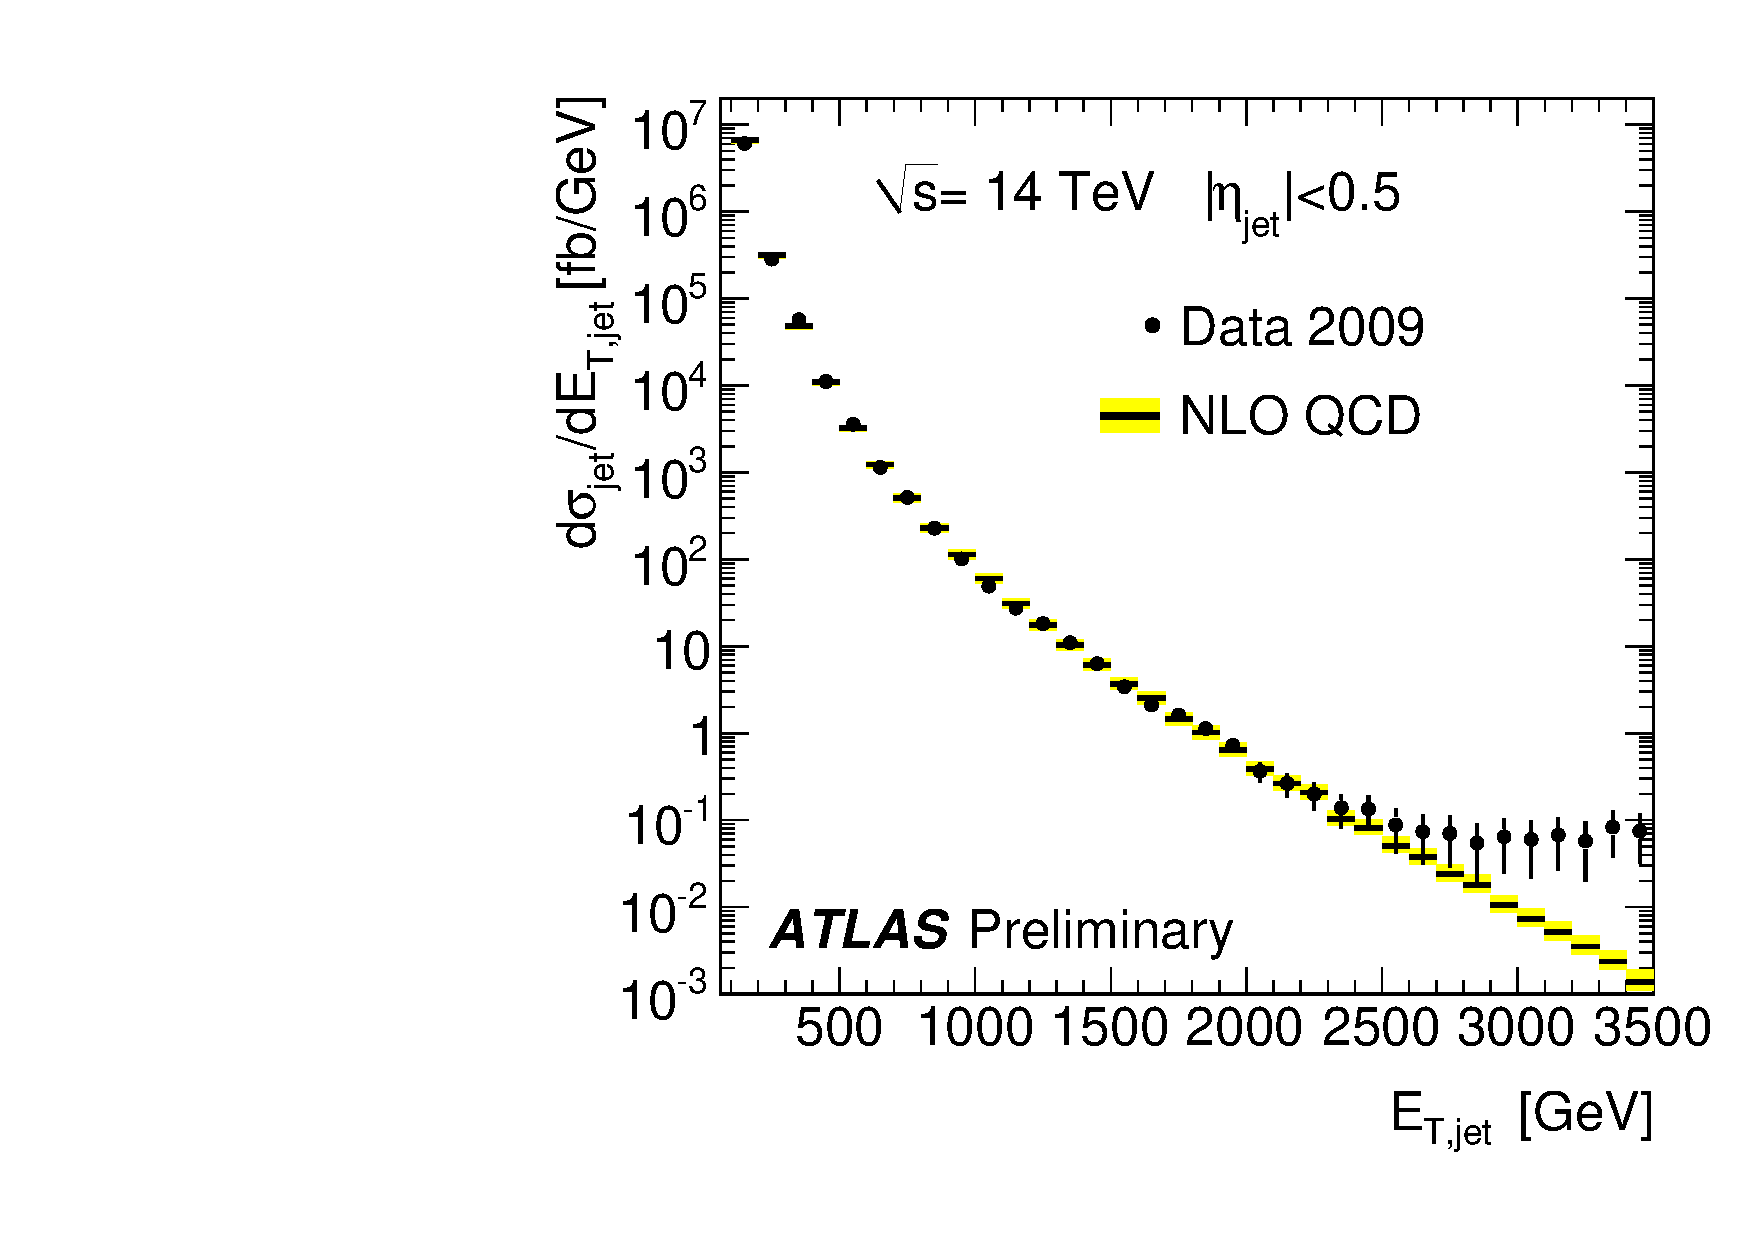
\includegraphics[width=8.0cm]{FigureExample}
  \caption{An example figure.}
  \label{fig:example}
\end{figure}

\section{Results}

This is the section where you present the results from the previous section. Data
should be compared with any theoretical predictions. Again, figures and tables
should be used as necessary. Be sure to include a discussion on how you estimate
your experimental uncertainties and how you propagate these uncertainties into
your results. 

%
%%%%%%%%%%%%%%%%%%%%%%%%%%%%%%%%%%%%%%%%%%%%%%%%%%%%%%%%%%%%%%%%%%%%%%%%%%%%%%%
% Discussion
%%%%%%%%%%%%%%%%%%%%%%%%%%%%%%%%%%%%%%%%%%%%%%%%%%%%%%%%%%%%%%%%%%%%%%%%%%%%%%%
%
\section{Discussion}
This is an extension of the section 5. Here you summarize the important results
and present your discussion of what the experiment shows and its significance.
Put the results into the context of the theory or a model.
This could be the section where one could discuss any future plans and new ideas.
This is a good place to discuss systematical uncertainties. 


%
%%%%%%%%%%%%%%%%%%%%%%%%%%%%%%%%%%%%%%%%%%%%%%%%%%%%%%%%%%%%%%%%%%%%%%%%%%%%%%%
% Summary and conclusion
%%%%%%%%%%%%%%%%%%%%%%%%%%%%%%%%%%%%%%%%%%%%%%%%%%%%%%%%%%%%%%%%%%%%%%%%%%%%%%%
%
\section{Summary and conclusion}

Reiterate the main points of the paper and the primary results and
conclusions.

Note that many readers look mostly at the title, abstract and
conclusion. The conclusion should be interesting enough to
make them want to read the whole paper.
It is not good style to just repeat the abstract.


%
%%%%%%%%%%%%%%%%%%%%%%%%%%%%%%%%%%%%%%%%%%%%%%%%%%%%%%%%%%%%%%%%%%%%%%%%%%%%%%%
% Acknowledgements
%%%%%%%%%%%%%%%%%%%%%%%%%%%%%%%%%%%%%%%%%%%%%%%%%%%%%%%%%%%%%%%%%%%%%%%%%%%%%%%
%
\section{Acknowledgements}
%
\begin{thebibliography}{99}
\bibitem{ref:cdfhyp} 
T.~Aaltonen {\it et al.}~(CDF Collaboration), Phy. Rev. D 86, 012002 (2012).
\end{thebibliography}
%
\end{document}

